\section{Introduction and Motivation}\label{sec:intro}
The data engineering domain has expanded monumentally over the past decade, thanks to the emergence of Machine Learning (ML) and Artificial Intelligence (AI). Data is no longer categorized as Gigabytes (GB) or Megabytes (MB), files, or databases but as terabytes or abstract data stores. It takes a considerable amount of developer time for pre-processing when a better use of time would be designing and implementing deep learning or machine learning models. The increasing amount of connected internet devices and social media results in data growing at parabolic or exponential rates.  Therefore, improving performance is critical to continuing to build pipelines that support the development of optimized AI/ML training and inference.

The exponential growth in data volume and complexity poses significant challenges across various scientific domains, particularly in genomics, climate modeling, astronomy, and neuroscience. For instance, the 1000 Genomes project and the Cancer Genome Atlas alone utilize nearly five terabases of data\cite{McKenna2010The}. The TSE search terabase alone consumes a substantial 50.4 TB in size. This can be understood by considering that a single genome sequence alone can generate approximately 200 GB of data\cite{genomefaq:online}. Consequently, by 2025, it would be necessary to store the genome sequences of the entire world, amounting to a staggering 40 exabytes of storage.

Similar challenges exist in astronomy. Faaique (2024) highlights the difficulties associated with processing and analyzing astronomical data and proposes cloud computing and cloud storage as potential solutions\cite{faaique} due to the immense data size and scale involved. Fox and Fathkouhi (2024) further introduce AstroMAE, the first application of a Mask Encoder on astronomical data\cite{Fathkouhi2024}. This application utilizes a dataset comprising 659,857 images with a resolution of 64 × 64 pixels and five color bands, resulting in approximately 54 GB of data with 10.4 million learnable parameters.  Fox (2025) delves into the challenges astronomers face when attempting to execute inference on foundational models on large astronomical images using standalone devices. It highlights the limitations imposed by memory and resource constraints on such devices\cite{Staylor2024cosmic}.

Decomposing complex problems represented by large datasets can be challenging and demands both scalable and efficient solutions. Machine Learning and Artificial Intelligence have revolutionized data analysis, allowing researchers to extract valuable insights that were previously unattainable. This leads to more robust and reliable results than possible with the previously available tools.

A crucial aspect of these solutions is the use of analytical engines that run on High-Performance Computing (HPC) clusters for training Large Language Models (LLMs) \cite{abeykoon2020data}. However, a significant challenge with this approach is that frameworks like Pandas, NumPy, and PyTorch are not directly compatible with technologies such as MPI, UCC/UCX, or Open Fabric Interfaces (OFI). 

Between 2005 and 2015, JVM frameworks and languages revolutionized Big Data with sophisticated processing and analysis. Over the past decade, however, Python has seen increased adoption and usage, surpassing Java and JVM usage, according to Google Trends.  Figure \ref{fig:javapythonadoption} shows Java versus Pythons based on reported Google trends from 2019 to 2025.  

\begin{figure}[ht]
    \begin{center}
    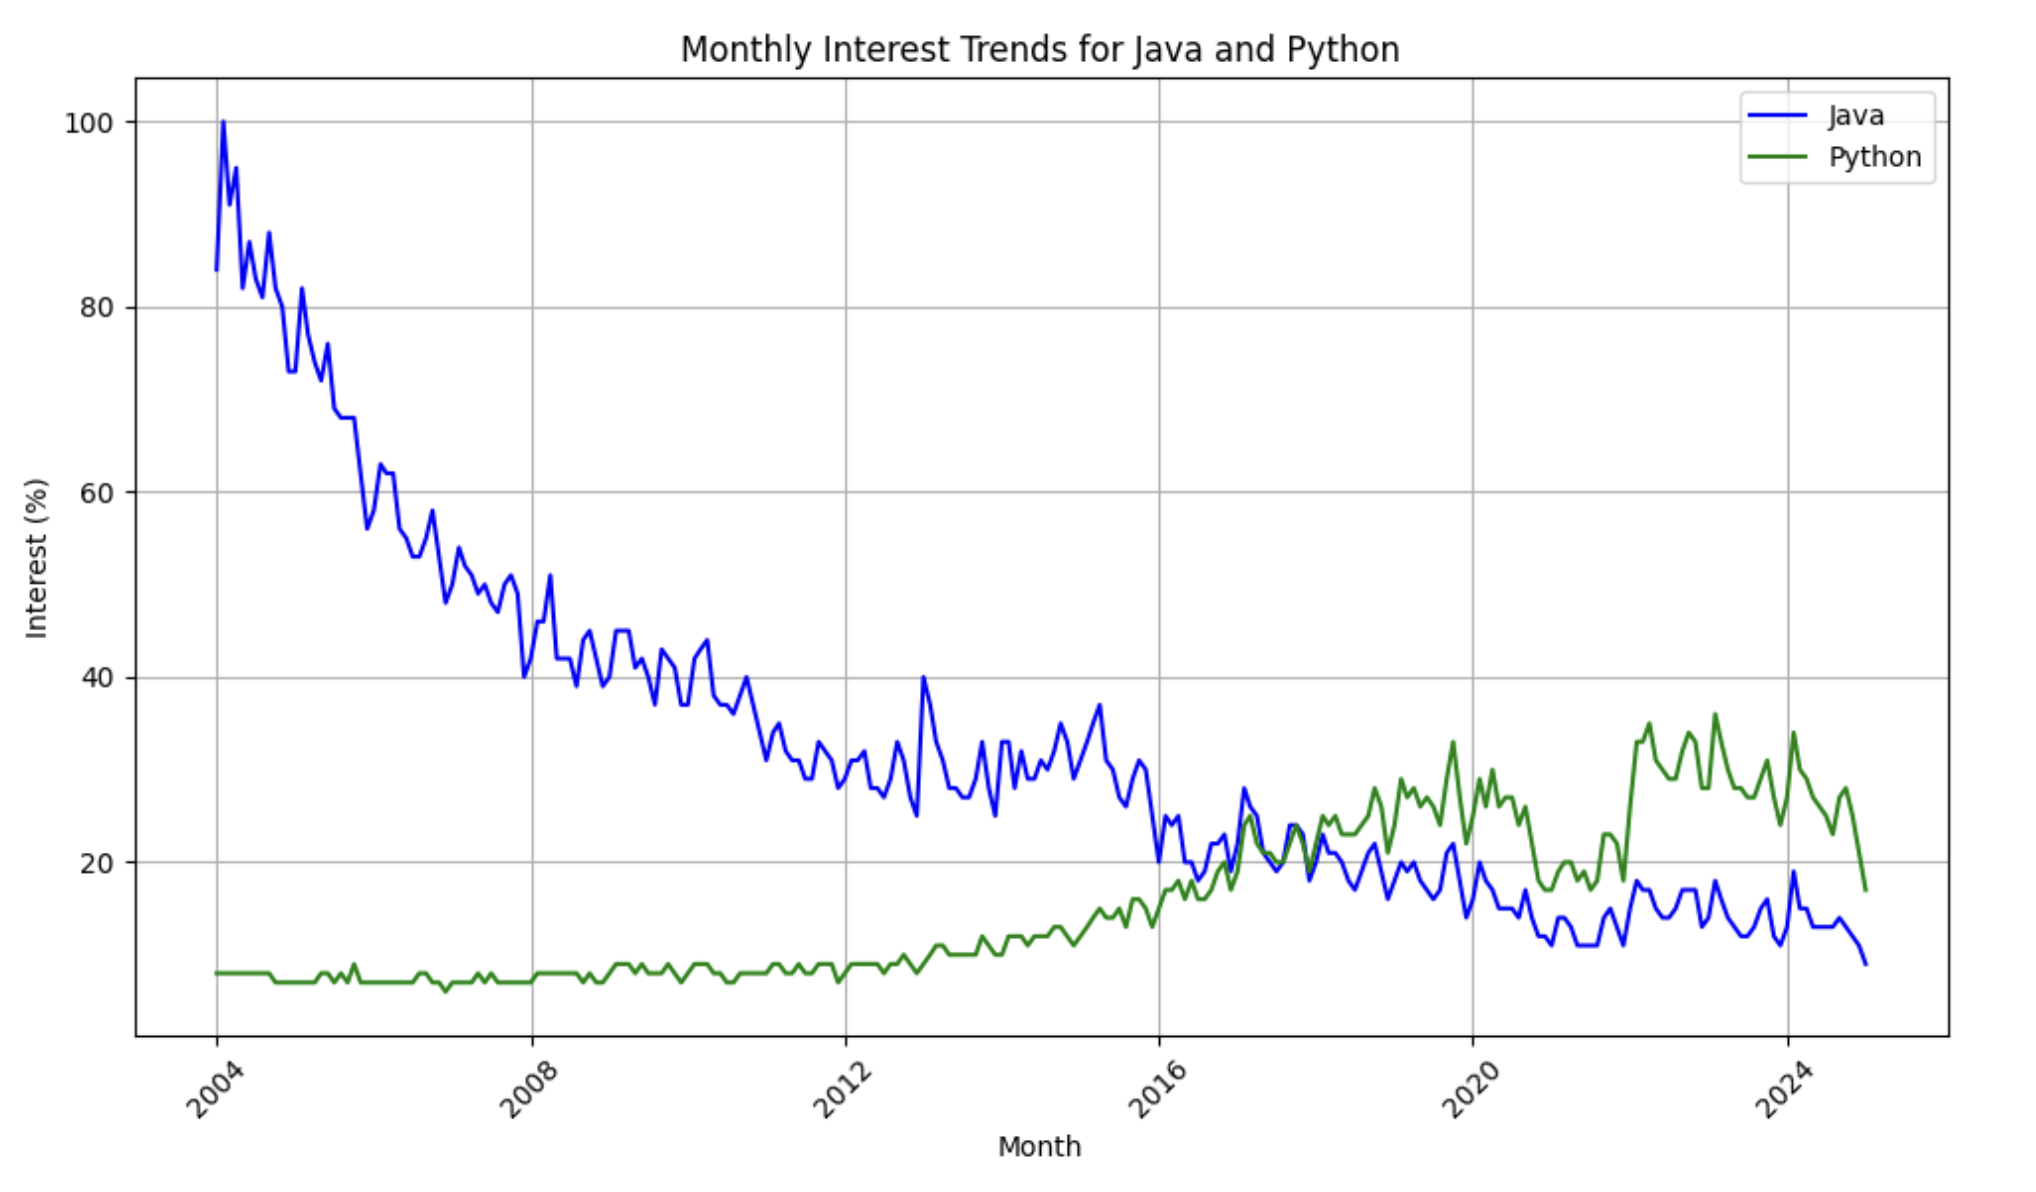
\includegraphics[width=\linewidth]{source/Figure/pythonjavainterest.png}
    \end{center}
    \caption{Java/Python Dominance}
    \label{fig:javapythonadoption}
\end{figure}

Python's dominance can be attributed to functional APIs such as Pandas, Modin, and Dask, a shallow learning curve, and user experience\cite{pererathesis}.  A key benefit of Python is it can interface directly with C/C++ or other native runtimes. Frameworks such as Pandas are not optimized with HPC-compute kernels.  Therefore, bindings such as Cython, which allow access to C++, can be used to create high-performance APIs for high-performance kernels available in HPC clusters such as UVA's Rivanna Supercomputer\cite{shan2022hybrid}.

The rise of Big Data and cloud computing, which began in the early 2000s, played a pivotal role in the emergence of modern artificial intelligence and machine learning. Machine learning and deep learning applications rely heavily on large, predetermined, and preprocessed datasets\cite{abeykoon2020data}. The exponential growth of data has posed significant challenges, particularly in terms of traditional storage and the need for efficient data exchange between distributed storage locations. Cloud computing services, such as Amazon Web Services (AWS), offer innovative solutions to these challenges by providing shared resources, including computing, storage, and analytics\cite{islamBigData}.

Function as a Service (FaaS) is a rapidly evolving paradigm in cloud computing applications. In FaaS, users focus on writing code that is broken down into individual functions. This approach allows users to concentrate on the application code itself, rather than the deployment and management of the underlying compute and storage infrastructure. Serverless functions also offer elasticity and fine-grained billing capabilities. However, serverless does not currently support efficient communication in the form of message passing for large-scale parallel data processing applications, such as Cylon\cite{copik2023fmi}. To address this limitation, Network Address Translation (NAT) in the form of TCP Hole Punching presents a high-performance and cost-effective alternative to other approaches, such as object or in-memory storage\cite{moyer2021punching}.

In this paper, we’ll delve into the concept of Cylon, a runtime engine designed to optimize the execution of deep learning applications in both high-performance computing (HPC) and cloud environments. We’ll explore the advantages of executing workloads within Docker containers on AWS using ECS tasks or managed Docker, and discuss how this approach can be extended to HPC environments utilizing Singularity or Apptainer.

We’ll then demonstrate the seamless integration of Docker execution environments with bare metal servers, showcasing that the runtime semantics are remarkably similar to those of native Docker containers, with minimal performance trade-offs.

Next, we’ll address the challenges associated with large-scale parallel execution on AWS and present the FMI library as a proof of concept for executing Cylon preprocessing and inference on FaaS environments. By demonstrating the library’s effectiveness, we’ll highlight its applicability to scientific domains, particularly astronomy.  We'll discuss costs associated with FaaS execution to illustrate the relevance and novelty of this approach compared to serverful execution in traditional HPC environments.

Finally, we’ll emphasize the potential of this work to revolutionize scientific research and data analysis in various fields

